%!/usr/bin/env latex
\documentclass[]{article}

%% Enhanced graphical abilities
\usepackage[pdftex]{graphicx}

%% TiKZ
\usepackage{tikz}
\usetikzlibrary{trees}

%% PDFTEX
\usepackage[pdftex]{hyperref}

\title{Example Game Trees with Tikz}
\author{Jeffrey Arnold}

\usepackage[latin1]{inputenc}
\usepackage{tikz}
\usetikzlibrary{trees}

\usepackage{amsfonts}% to get the \mathbb alphabet
\newcommand{\field}[1]{\ensuremath{\mathbb{#1}}}
\newcommand{\R}{\field{R}}

\begin{document}

\maketitle{}

Some game trees I drew with Tikz in PSC 584.

\begin{figure}[ht]\centering
    
    \tikzstyle{level 1}=[level distance=1cm, sibling distance=3cm]
    \tikzstyle{level 2}=[level distance=1cm, sibling distance=2cm]
    \tikzstyle{action} = [circle, minimum width=3pt, fill]
    \tikzstyle{terminal} = []
  
  \begin{tikzpicture}[grow=down, scale=2]
    \node[action, label=above: {C}] {} 
    child { 
      node[terminal, label=below: {$1,2$}] {} 
      edge from parent node[left] {$O$} 
    }
    child { 
      node[action, label=right: {I}] {} 
      child { 
        node[terminal, label=below: {$2,1$}] {} 
        edge from parent node[left] {$R$} }
      child { 
        node[terminal, label=below: {$0,x$}] {} 
        edge from parent node[right] {$\lnot R$} 
      } 
      edge from parent node[right] {$E$}
    };
  \end{tikzpicture}
  
  \caption{Simple Extensive Form Game}
\label{fig:alfa}
\end{figure}

\begin{figure}[ht]\centering
  
  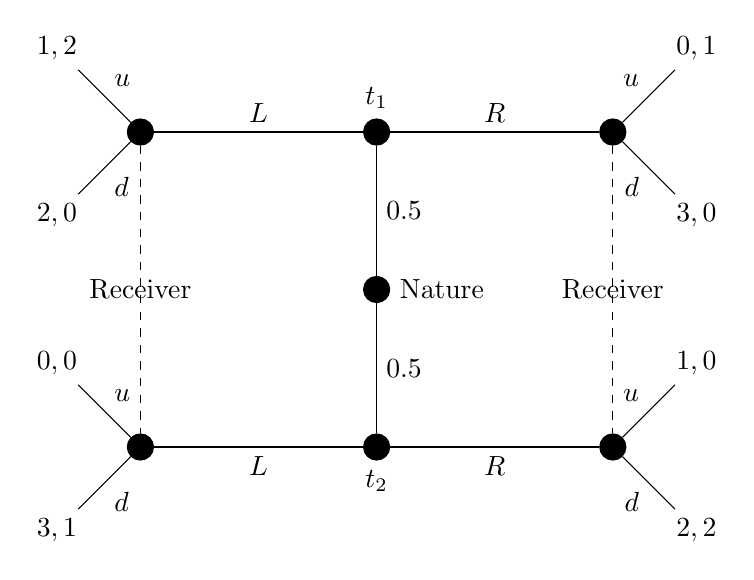
\begin{tikzpicture}[node distance=1.5cm]
    \tikzstyle{action}=[draw,circle,fill]; \tikzstyle{end}=[]; \node
    (0) [action,label=right:Nature] at (0,0) {};

    \node (1) [action,label=above:$t_{1}$] at (0,2) {}; \node (2)
    [action,label=below:$t_{2}$] at (0,-2) {};

    \node (3) [action] at (3,2) {};
     \node (3a) [end,above right of=3] {$0,1$} ;
     \node (3b) [end,below right of=3] {$3,0$} ;


    \node (4) [action] at (-3,2) {};
     \node (4a) [end,above left of=4] {$1,2$} ;
     \node (4b) [end,below left of=4] {$2,0$} ;


    \node (5) [action] at (3,-2) {};
     \node (5a) [end,above right of=5] {$1,0$} ;
     \node (5b) [end,below right of=5] {$2,2$} ;


    \node (6) [action] at (-3,-2) {};
     \node (6a) [end,above left of=6] {$0,0$} ;
     \node (6b) [end,below left of=6] {$3,1$} ;


    \path (0) edge node[right] {0.5} (1) edge node[right] {0.5} (2)
    (4) edge [dashed] node[] {Receiver} (6) (3) edge [dashed] node[]
    {Receiver} (5) (1) edge node[above] {$R$} (3) edge node[above]
    {$L$} (4) (2) edge node[below] {$R$} (5) edge node[below] {$L$}
    (6) (3) edge node[above left] {$u$} (3a) edge node[below left]
    {$d$} (3b) (4) edge node[above right] {$u$} (4a) edge node[below
    right] {$d$} (4b) (5) edge node[above left] {$u$} (5a) edge
    node[below left] {$d$} (5b) (6) edge node[above right] {$u$} (6a)
    edge node[below right] {$d$} (6b);
  \end{tikzpicture}
  
  \caption{Game tree from Gibbons Problem 4.3 (a)}
\label{fig:gibbons43a}
\end{figure}

\begin{figure}[ht]
\centering
  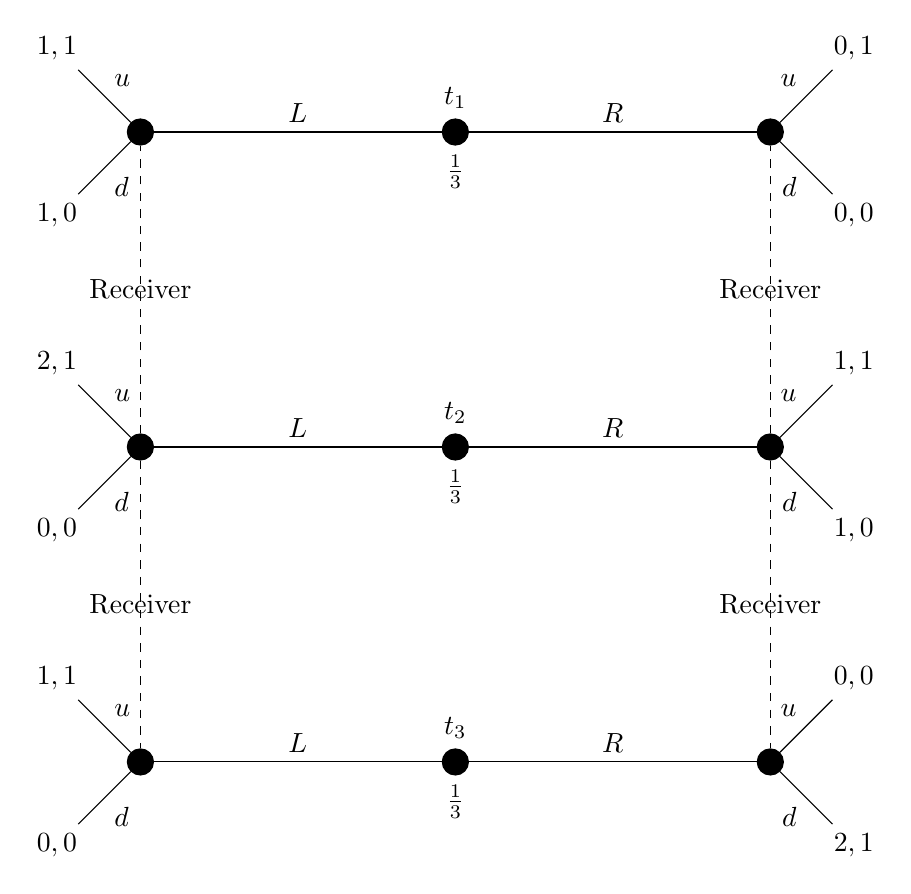
\begin{tikzpicture}[node distance=1.5cm,scale=2]
    \tikzstyle{action}=[draw,circle,fill]; 
    \tikzstyle{end}=[];

    \node (1) [action,label=above:$t_{1}$,label=below:$\frac{1}{3}$]
    at (0,2) {}; \node (1R) [action] at (2,2) {}; \node (1Ru)
    [end,above right of=1R] {$0,1$}; \node (1Rd) [end,below right
    of=1R] {$0,0$};

    \node (1L) [action] at (-2,2) {}; \node (1Lu) [end,above left
    of=1L] {$1,1$}; \node (1Ld) [end,below left of=1L] {$1,0$};

    \node (2) [action,label=above:$t_{2}$,label=below:$\frac{1}{3}$]
    at (0,0) {}; \node (2R) [action] at (2,0) {}; \node (2Ru)
    [end,above right of=2R] {$1,1$}; \node (2Rd) [end,below right
    of=2R] {$1,0$};
  
    \node (2L) [action] at (-2,0) {}; \node (2Lu) [end,above left
    of=2L] {$2,1$}; \node (2Ld) [end,below left of=2L] {$0,0$};

    \node (3) [action,label=above:$t_{3}$,label=below:$\frac{1}{3}$]
    at (0,-2) {};

    \node (3R) [action] at (2,-2) {}; \node (3Ru) [end,above right
    of=3R] {$0,0$}; \node (3Rd) [end,below right of=3R] {$2,1$};

    \node (3L) [action] at (-2,-2) {}; \node (3Lu) [end,above left
    of=3L] {$1,1$}; \node (3Ld) [end,below left of=3L] {$0,0$};

    \path (1) edge node[above] {$R$} (1R) edge node[above] {$L$} (1L)
    (2) edge node[above] {$R$} (2R) edge node[above] {$L$} (2L) (3)
    edge node[above] {$R$} (3R) edge node[above] {$L$} (3L) (1L) edge
    node[above right] {$u$} (1Lu) edge node[below right] {$d$} (1Ld)
    (2L) edge node[above right] {$u$} (2Lu) edge node[below right]
    {$d$} (2Ld) (3L) edge node[above right] {$u$} (3Lu) edge
    node[below right] {$d$} (3Ld)

    (1R) edge node[above left] {$u$} (1Ru) edge node[below left] {$d$}
    (1Rd) (2R) edge node[above left] {$u$} (2Ru) edge node[below left]
    {$d$} (2Rd) (3R) edge node[above left] {$u$} (3Ru) edge node[below
    left] {$d$} (3Rd)

    (2L) edge[dashed] node {Receiver} (1L) edge[dashed] node
    {Receiver} (3L) (2R) edge[dashed] node {Receiver} (1R)
    edge[dashed] node {Receiver} (3R) ;
  \end{tikzpicture}
  
  \caption{Game tree from Gibbons Problem 4.3 (b)}
\label{fig:gibbons43b}
\end{figure}

\begin{figure}
     \centering
     \tikzstyle{level 1}=[level distance=1cm, sibling distance=6cm]
     \tikzstyle{level 2}=[level distance=2cm, sibling distance=3cm]
     \tikzstyle{level 3}=[level distance=2cm, sibling distance=1cm]
     \tikzstyle{action} = [circle, fill]
     \tikzstyle{root} = [draw, circle]
     \tikzstyle{terminal} = []
     
     \begin{tikzpicture}[grow=down, scale=1]
       \node [root, label=above: {$N$}] {} 
       child { 
         node (L) [action, label=above: {$1$}] {} 
         child {
           node (LA) [action, label=above: {$2$}] {}
           child { 
             node  [terminal] {$(.,1)$}
             edge from parent node[above left] {$a_1$} 
           }
           child { 
             node  [terminal] {$(., 1)$}
             edge from parent node[left] {$a_2$} 
           }
           child { 
             node  [terminal] {$(., 0)$}
             edge from parent node[above right] {$a_3$} 
           }
           edge from parent node[above left] {$A$}
         }
         child {
           node (LB) [action, label=above: {$2$}] {}
           child { 
             node  [terminal] {}
             edge from parent node[above left] {} 
           }
           child { 
             node  [terminal] {}
             edge from parent node[left] {} 
           }
           edge from parent node[above right] {$B$}
         }
         edge from parent node[above left] {$p$} node[below right] {$L$}
       }
      child { 
         node (R) [action, label=above: {$1$}] {} 
         child {
           node (RA) [action, label=above: {$2$}] {}
           child { 
             node  [terminal] {$(.,1)$}
             edge from parent node[above left] {$a_1$} 
           }
           child { 
             node  [terminal] {$(., 1)$}
             edge from parent node[left] {$a_2$} 
           }
           child { 
             node  [terminal] {$(., 0)$}
             edge from parent node[above right] {$a_3$} 
           }
           edge from parent node[above left] {$A$}
         }
         child {
           node (RB) [action, label=above: {$2$}] {}
           child { 
             node  [terminal] {}
             edge from parent node[above left] {} 
           }
           child { 
             node  [terminal] {}
             edge from parent node[left] {} 
           }
           edge from parent node[above right] {$B$}
         }
         edge from parent node[above right] {$1 - p$} node[below left] {$R$}
       }
      ;
      \path (RA) edge[dashed,bend right=15] (LA);
      \path (RB) edge[dashed,bend right=15] (LB);
   \end{tikzpicture}
  \caption{Example of a signaling game where $MBR(A) \neq \triangle BR(A)$.}
  \label{fig:p3}
\end{figure}

\begin{figure}[ht]
  \centering
  \tikzstyle{level 1}=[level distance=1cm, sibling distance=3cm]
  \tikzstyle{level 2}=[level distance=1cm, sibling distance=2cm]
  \tikzstyle{action} = [circle, fill]
  \tikzstyle{root} = [draw, circle]
  \tikzstyle{terminal} = []
     
  \begin{tikzpicture}[grow=down, scale=1]
    \node [root, label=above: {1}] {} 
    child { 
      node (a) [action] {} 
      child { 
        node[terminal, label=below: {$4,2$}] {} 
        edge from parent node[left] {$C$} 
      }
      child { 
        node[terminal, label=below: {$1,1$}] {} 
        edge from parent node[right] {$D$} 
      } edge from parent node[above left] {$A$}
    }
    child { 
      node (b) [action] {} 
      child { 
        node[terminal, label=below: {$5,1$}] {} 
        edge from parent node[left] {$C$} 
      }
      child { 
        node[terminal, label=below: {$2,2$}] {} 
        edge from parent node[right] {$D$} 
      } edge from parent node[above right] {$B$}
    };
    %% Add information set 
    \path (a) edge[dashed] node[above] {$2$} (b) ;
  \end{tikzpicture}
  \caption{Game Tree for Problem 6(b)}
\end{figure}

\begin{figure}
     \centering
     \tikzstyle{level 1}=[level distance=1cm, sibling distance=6cm]
     \tikzstyle{level 2}=[level distance=2cm, sibling distance=3cm]
     \tikzstyle{level 3}=[level distance=1.5cm, sibling distance=1.5cm]
     \tikzstyle{action} = [circle, fill]
     \tikzstyle{root} = [draw, circle]
     \tikzstyle{terminal} = []
     
     \begin{tikzpicture}[grow=down, scale=1]
       \node [root, label=above: {$N$}] {} 
       child { 
         node (T) [action, label=above: {$1$}] {} 
         child { 
           node (TA) [action, label=above: {$2$}] {}
           child {
             node [terminal] {$4,2$}
             edge from parent node[above left] {$C$}
           }
           child {
             node [terminal] {$1,1$}
             edge from parent node[above right] {$D$}
           }
           edge from parent node[above left] {$A$} node[below] {$a$}
         }
         child { 
           node (TB) [action] {}
           child {
             node [terminal] {$5,1$}
             edge from parent node[above left] {$C$}
           }
           child {
             node [terminal] {$2,2$}
             edge from parent node[above right] {$D$}
           }
           edge from parent node[above right] {$B$} node[below] {$b$}
         }
         edge from parent node[above left] {$T$} node[below right] {$p$}
       }
       child { 
         node (F) [action, label=above: {$1$}] {} 
         child { 
           node (FB) [action] {}
           child {
             node [terminal] {$5,1$}
             edge from parent node[above left] {$C$}
           }
           child {
             node [terminal] {$2,2$}
             edge from parent node[above right] {$D$}
           }
           edge from parent node[above left] {$B$} node[below] {$a$}
         }
         child { 
           node (FA) [action, label=above: {$2$}] {}
           child {
             node [terminal] {$4,2$}
             edge from parent node[above left] {$C$}
           }
           child {
             node [terminal] {$1,1$}
             edge from parent node[above right] {$D$}
           }
           edge from parent node[above right] {$A$} node[below] {$b$}
         }
         edge from parent node[above right] {$F$} node[below left] {$1 -p$}
       };
       %% Add information set 
       \path (T) edge[dashed] (F);
       \path (TA) edge[dashed,bend left=15] (FB);
       \path (TB) edge[dashed,bend left=15] (FA);
  \end{tikzpicture}
  \caption{Alternate extensive form game tree for Problem 6 (c)}
\end{figure}

\begin{figure}
     \centering
     \tikzstyle{level 1}=[level distance=2cm, sibling distance=3cm]
     \tikzstyle{level 2}=[level distance=1cm, sibling distance=1cm]
     \tikzstyle{level 3}=[level distance=1cm, sibling distance=0.5cm]
     \tikzstyle{action} = [circle, fill]
     \tikzstyle{root} = [draw, circle]
     \tikzstyle{terminal} = []
     
     \begin{tikzpicture}[grow=down, scale=1]
       \node [root, label=above: {$N$}] {} 
       child { 
         node (L) [action, label=above: {$1$}] {} 
         child {
           node (LA) [terminal, label=above: {$2$}] {$g \in \R$}
           edge from parent node[above left] {$Y$}
         }
         child {
           node (LA) [terminal, label=above: {$2$}] {$g \in \R$}
           edge from parent node[above right] {$N$}
         }
         edge from parent node[above left] {$(H, G)$} node[below right] {$\frac{1}{3}$}
       }
       child { 
         node (L) [action, label=above: {$1$}] {} 
         child {
           node (LA) [terminal, label=above: {$2$}] {$g \in \R$}
           edge from parent node[above left] {$Y$}
         }
         child {
           node (LA) [terminal, label=above: {$2$}] {$g \in \R$}
           edge from parent node[above right] {$N$}
         }
         edge from parent node[left] {$(M, G)$} node[right] {$\frac{1}{6}$}
       }
       child { 
         node (L) [action, label=above: {$1$}] {} 
         child {
           node (LA) [terminal, label=above: {$2$}] {$g \in \R$}
           edge from parent node[above left] {$Y$}
         }
         child {
           node (LA) [terminal, label=above: {$2$}] {$g \in \R$}
           edge from parent node[above right] {$N$}
         }
         edge from parent node[right] {$(M, B)$} node[left] {$\frac{1}{6}$}
       }
       child { 
         node (L) [action, label=above: {$1$}] {} 
         child {
           node (LA) [terminal, label=above: {$2$}] {$g \in \R$}
           edge from parent node[above left] {$Y$}
         }
         child {
           node (LA) [terminal, label=above: {$2$}] {$g \in \R$}
           edge from parent node[above right] {$N$}
         }
         edge from parent node[above right] {$(L, B)$} node[below left] {$\frac{1}{3}$}
       }
       ;
      %\path (RA) edge[dashed,bend right=15] (LA);
      %\path (RB) edge[dashed,bend right=15] (LB);
   \end{tikzpicture}
  \caption{Game tree for game in Problem 2}
  \label{fig:p2}
\end{figure}


\end{document}
